\documentclass[10pt, journal]{IEEEtran}
\usepackage{lipsum}
\usepackage{cite}
\usepackage{url}
\usepackage{graphicx}


\author{\IEEEauthorblockN{Remco Aarts}, 
 \IEEEauthorblockN{Jeroen van den Akker}, 
 \IEEEauthorblockN{Robert Delmaar}, 
 \IEEEauthorblockN{Bas Janssen},
 \IEEEauthorblockN{Addie Perenboom},
 \IEEEauthorblockN{Dimitri Waard}}

%\author{Remco Aarts, Jeroen van den Akker, Robert Delmaar, Bas Janssen, Addie Perenboom, Dimitri Waard}

\title{Decentralized multi-robot logistics}

\begin{document}
\maketitle

\begin{abstract}
This paper details the design and implementation of a decentralized multi-robot logistics system. Both the hardware design and the software design and implementation are expended upon below.
\end{abstract}
\begin{IEEEkeywords}

\end{IEEEkeywords}

\section{Introduction}
The decentralized multi-robot logistics project is one of the main projects of the Adaptive Robotics Minor at Fontys Hogeschool Engineering, in the 2016-2017 academic year. The goal of this project is to develop a system, both hardware and software, that is capable of transporting product between a warehouse and production locations in an Industry 4.0 setting. The system can be a replacement for a traditional conveyor belt, or can be used as a flexible addition to an existing conveyor system.

\section{Hardware}
The turtlebots must transport carriages from one point in a warehouse/factory to another point. In addition to this it was decided that the turtlebots had to be able to transfer carriages from one bot to another. A morphological chart was used to create multiple solutions for this task. The solutions that were most promising and realistic were worked out with more detail. Initially the turtlebots were meant to have multiple specializations. These specializations were also in the morphological chart. Two of these specializations were chosen, but in the end, it was financially and time-wise not feasible to implement both specializations. Hence only one concept was realized.
\subsection{Stackup}
The position of the camera was moved to the front of the turtlebot, beneath the disk on top of which the laptop is placed. The system that hold the carriages and is capable of transferring the carriages is mounted on top of the disk above the laptop.
\begin{figure}[htp]
\centering
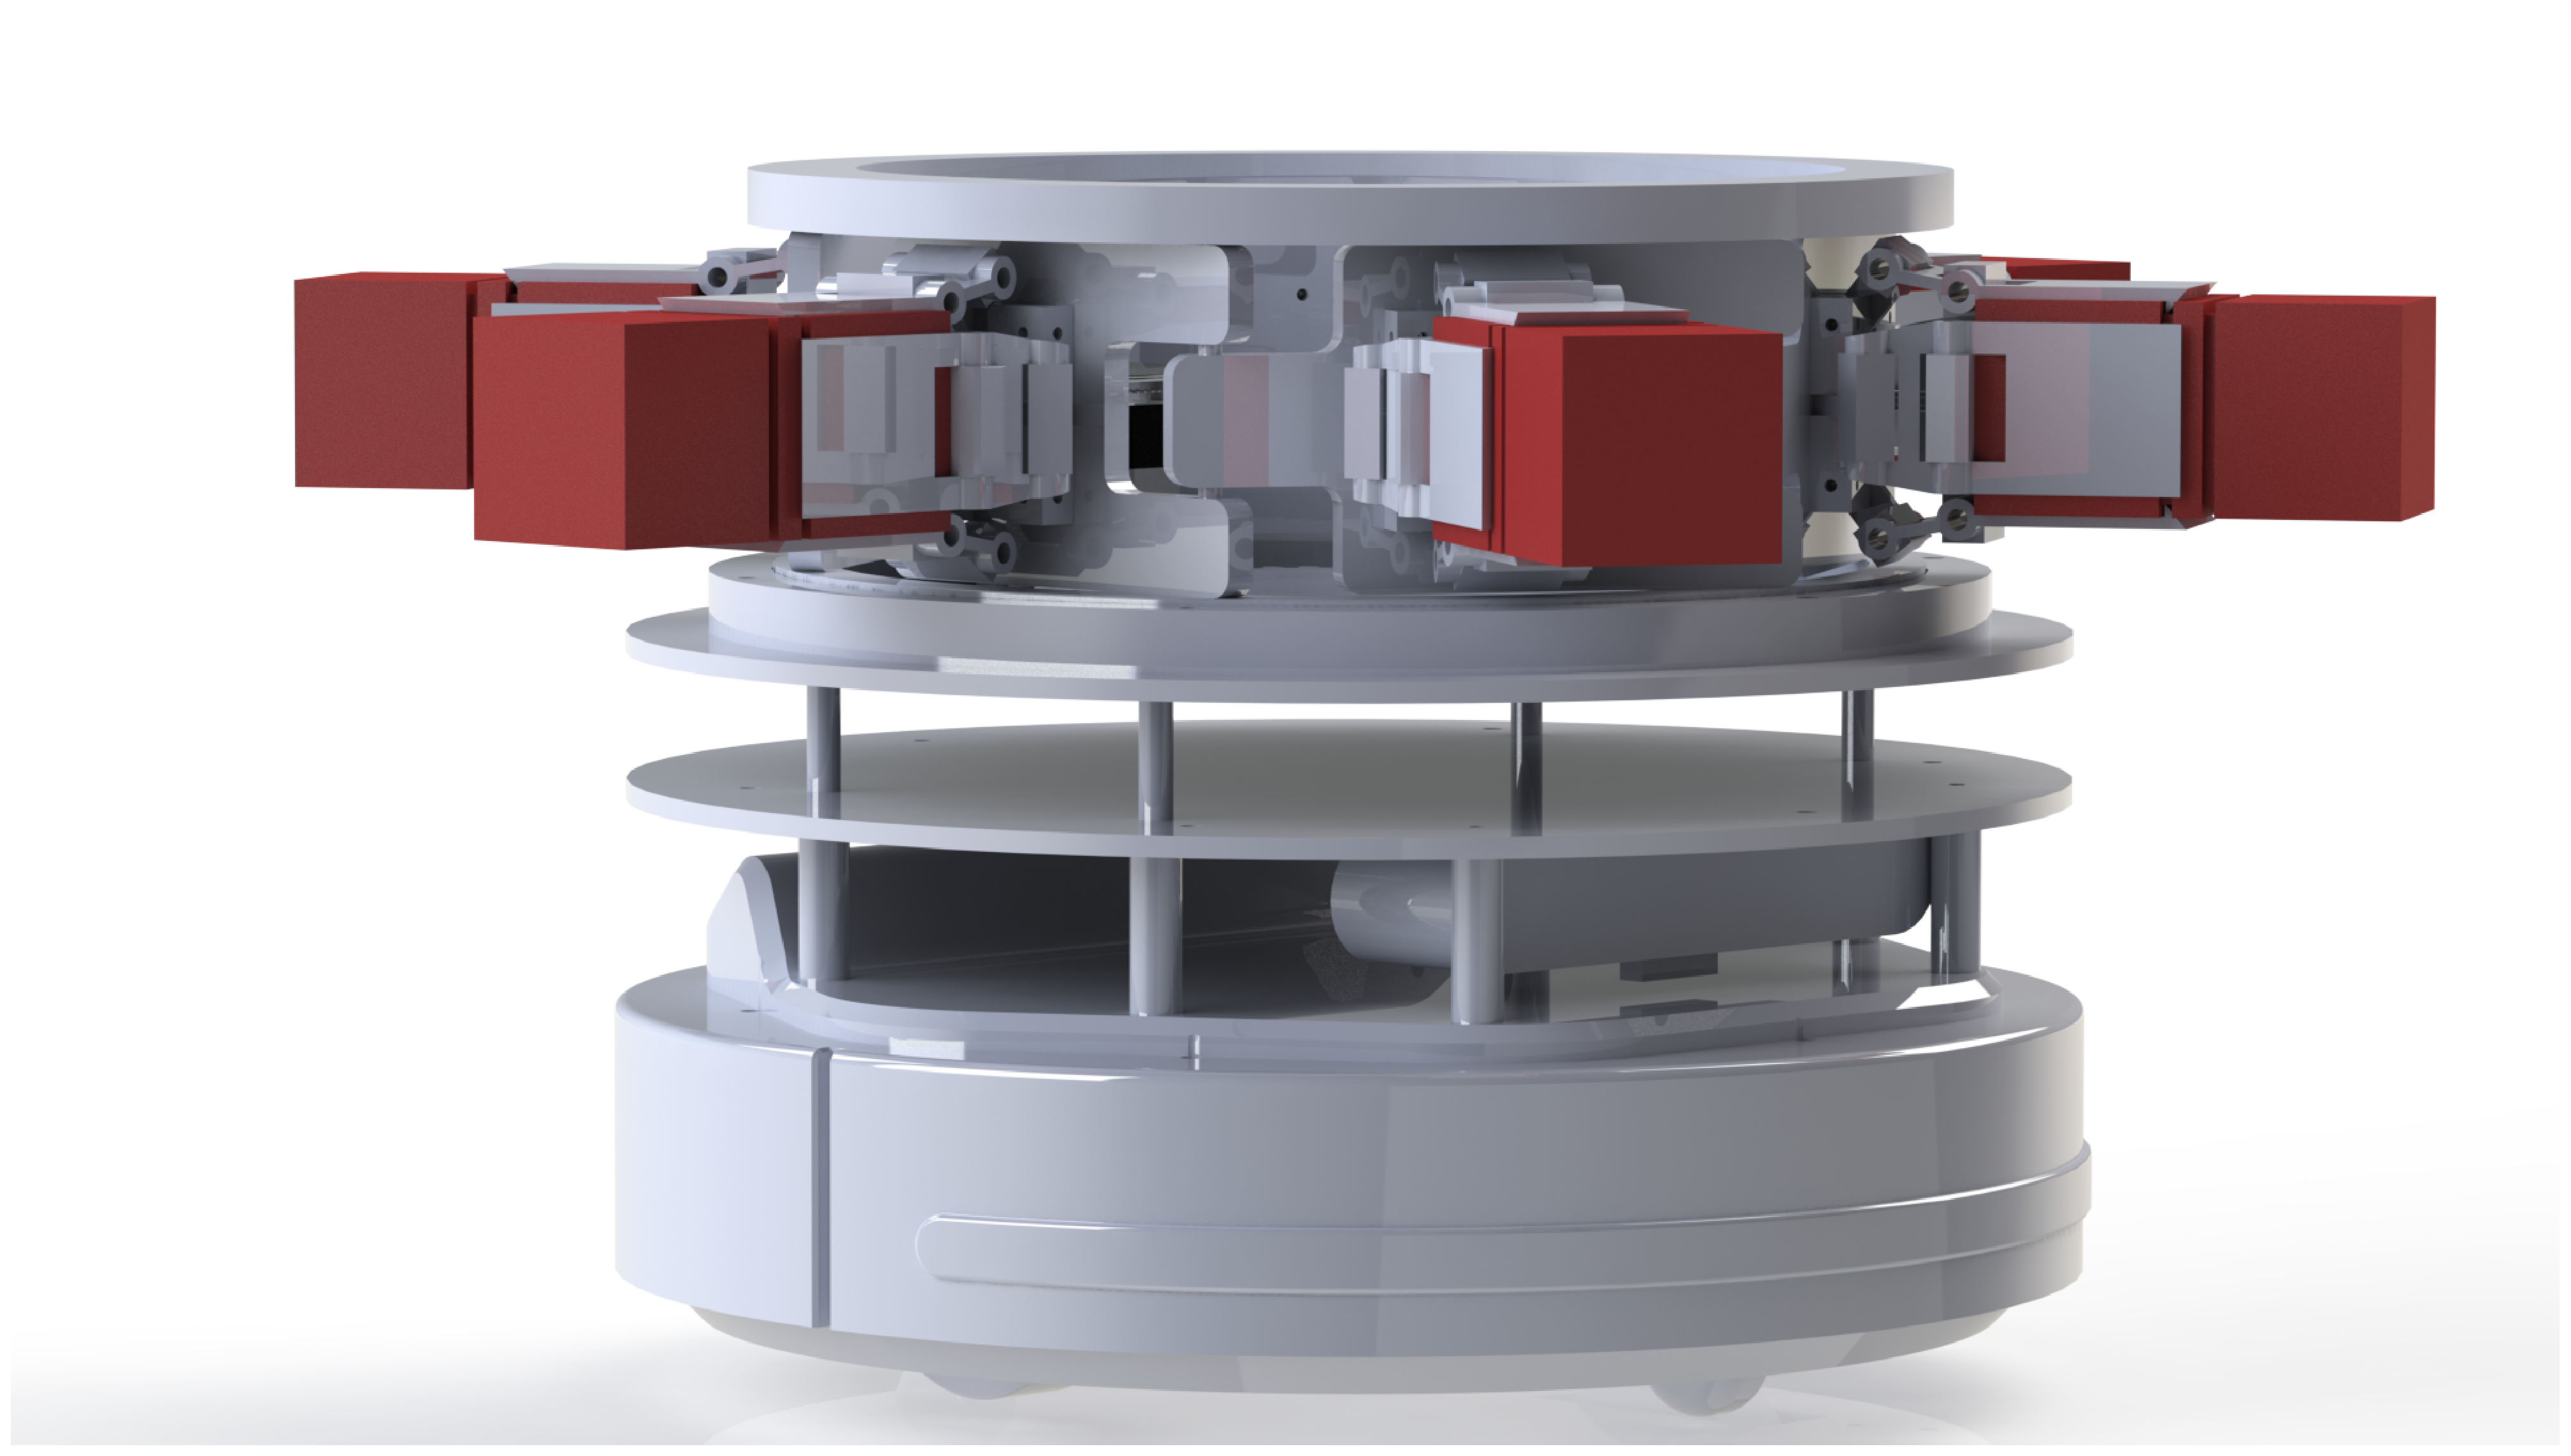
\includegraphics[width=\columnwidth]{turtle_design}
\caption{Mechanical Design}
\label{MechanicalDesign}
\end{figure}

Six grippers are mounted on the turtlebot, each can carry a single carriage. To align the carriages for transfer the grippers can revolve around the turtlebot. For this purpose, the grippers and a stepper motor are mounted on top of a Lazy Suzan bearing. A pinion on the motor and a gear make it possible for the bearing to revolve. A reed contact and a magnet are used to keep track of the position of the grippers instead of an encoder. A slip ring is used to keep the electrical cables from getting entangled or breaking lose because of the movement. This design is displayed in figure \ref{MechanicalDesign}.

\subsection{Gripper}
When a carriage is pushed into the gripper a plate with an axis attached to it will be pushed back. Pushing the plate back will cause the fingers to grip the carriage. The gripper will be mechanically locked by the axis, to be released by a servo. When released a spring pushes the plate back, causing the gripper to open. The carriages will be pushed into the carriage by driving the turtlebot against it. To get the alignment right the gripper is revolved around the turtlebot first.

The carriages are a standard size of 50*50*100mm and are intended to carry small parts such as bolts. A photograph of the gripper is shown in figure \ref{Gripper}.
\begin{figure}[htp]
\centering
\includegraphics[width=\columnwidth]{gripper}
\caption{Gripper}
\label{Gripper}
\end{figure}

\section{Software}
During this project a team of two students has developed the software making the decisions on the robots. This software is designed to receive commands from one or more workstations, and have to robots decide which robot should execute a command. The robots have the ability to request help from one another when more product have to be transported than a single robot can carry, or it is beneficial to transfer one or more products between two robots to get the products to their destination faster.

\subsection{Distance calulation}
The robots make decisions based on their available inventory space, and the distance between the robot and the goal. The distance of the planned path is calculated using equation \ref{eq_pathlength}. This means that for each point in the path, the distance to the next point is calculated. The length is the sum of these distances.
\begin{equation}
\label{eq_pathlength}
x = \sum\limits_{i=0}^j \sqrt{(y_i - y_{i+1})^2 + (x_i - x_{i+1})^2}
\end{equation}

\subsection{Multimaster-fkie}
All the robots in the group communicate with each other. As each robot is its own ROS master, the normal\cite{ROSMultipleMachines} way of using multiple machines in the ROS ecosystem is not viable. However, a package capable of communicating between multiple independent ROS masters has been developed at the Fraunhofer-Institut für Kommunikation, Informationsverarbeitung und Ergonomie FKIE, called multimaster-fkie \cite{Multimaster-fkie}. Using this package it is possible to synchronize one or more topics between one or more ROS masters. This project uses said functionality to synchronize the command and control topics for the robots between the robots and the workstations.

The multimaster package provides two nodes, namely master-discovery and master-sync. The master-discovery node uses a multicast address to find the other masters on the network, and this list of masters is passed to the master-sync node to synchronize the specified topics.
\subsection{Simulation}
To test the software during development a simulation in Gazebo has been configured\cite{MultipleRobots}. The simulation has been configured for four robots, because the computer systems available could not simulate more robots at the same time with reasonable performance. Four robots also allow for testing assistive operation and provide the capability to have multiple robots running multiple different commands.

Within this simulation, the complete robots are simulated in a fully simulated world. This means that the robots are subject to simulated physics, collisions are possible and the entire software stack for each robot is running. To complete the simulation, a virtual world has been build for the robots to move around in. This would consists of eight one by one by one meter cubes that represent obstacles. The cubes are spaced through out this virtual world.
\begin{figure}[htp]
\centering
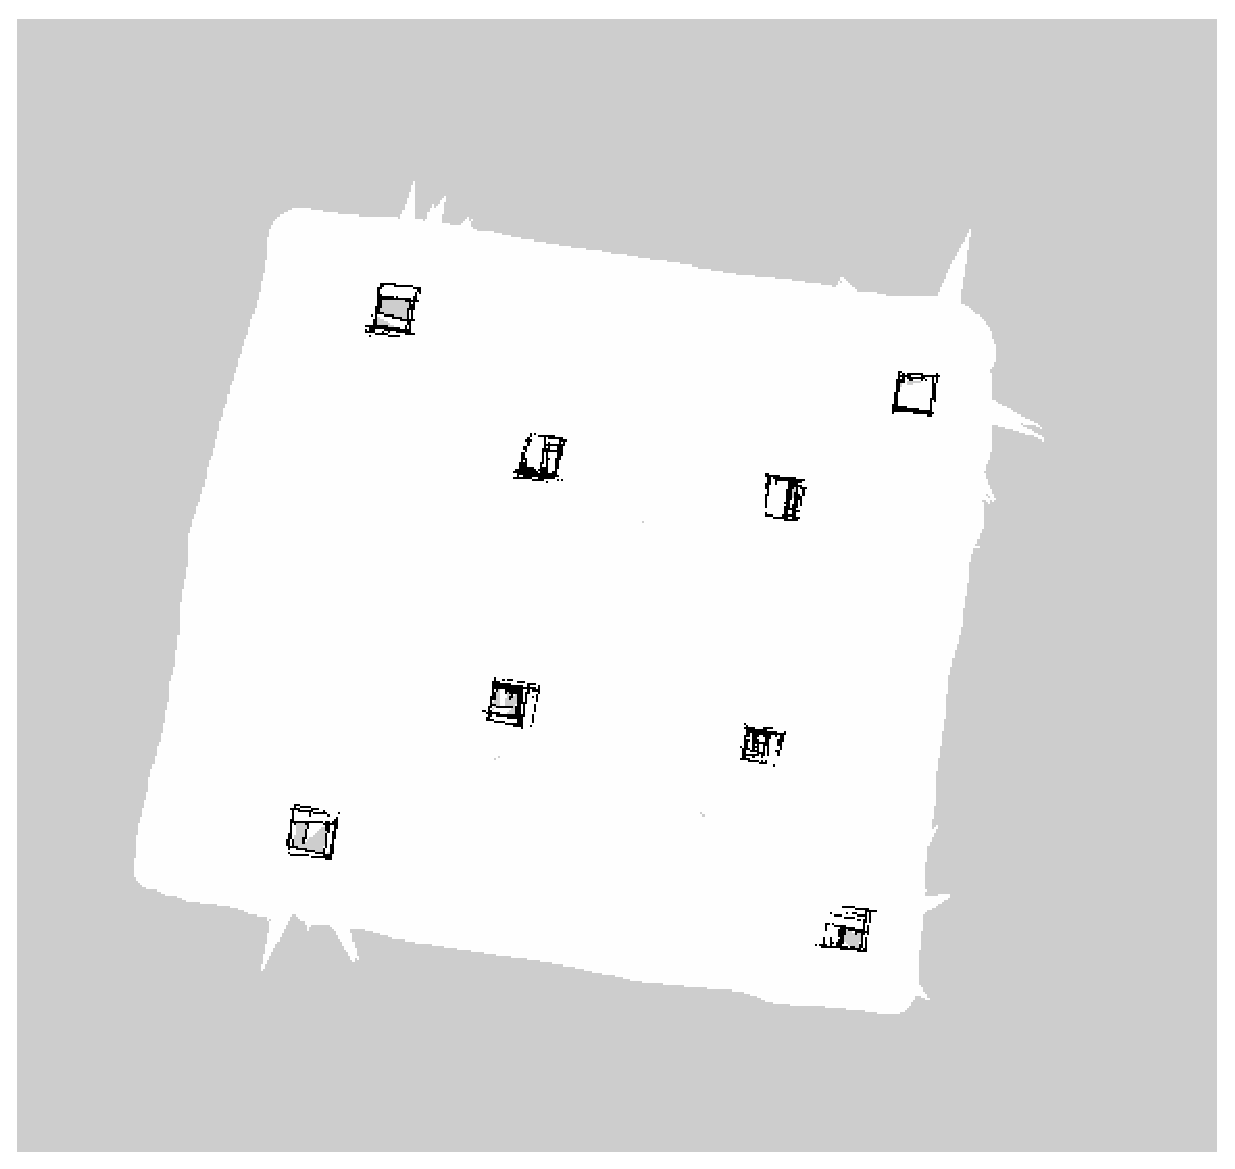
\includegraphics[width=\columnwidth]{gazebo_2}
\caption{Map of the simulated world}
\label{SimulatedWorldMap}
\end{figure}

Figure \ref{SimulatedWorldMap} shows the map of this virtual world generated with gmapping SLAM package\cite{SLAMGmapping}, and edited to expand the known area. The white area represents the know area, grey represents unknown and the black markings are the detected obstacles.
\subsection{Software scales to more robots}
The software has been designed to scale to an unlimited number of robots. The only requirement is that the systems running the robots have enough RAM to store all the information for the robots. The software has been tested in the simulation with four robots.
\subsection{Replace turtlebots}
During testing, it was determined that the turtlebots are not suitable for this application. The odometry of the turtlebots is lacking, and very error prone. The Orbbec Astra RGBD camera placed on the turtlebot is not very suitable as a simulated laserscanner, as the resolution and update rate are to low to provide detailed information. It is therefore recommended to replace the turtlebots with a more suitable robot platform if this system is to be taken further than the proof of concept phase.

\bibliographystyle{IEEEtran}
\bibliography{paper_multirobot_logistics}
\end{document}